
\section{What is Receive Side Scaling or RSS? \label{sectionRSSIntroduction}}
The multiple cores present on the current hardware can be used to scale the processing capability of a single node.
A packet arriving on the NIC is redirected to different cores for independent processing. This redirection may occur either
in software or hardware.
\begin{itemize}
        \item \textbf{Software} A master core receives all the packets and redirects it to multiple  worker cores. This redirection can happen in round robin or hash computation with header fields as key for the hash function (see Figure \ref{figPipeline}). 
The hash computation technique is preferred as packets of the same flow go to the same core giving better memory locality. This model is referred to as the  pipeline model of execution. 
       \item  \textbf{Hardware (on the NIC)} The hash computation on header fields happen on the NIC itself (see Figure \ref{figRTC}). This is known as Receive Side Scaling (RSS). The rest of the packet processing happens in software. The RSS computation in the context of 5G UPF uplink packet handling will be discussed.  
\end{itemize}
These alternative models of execution are discussed in Chapter \ref{chapterModelsofExecution}. 

\section{Standard RSS \label{sectionstandardRSS}}



The RSS hash for an incoming packet is computed on the transport and network layer headers. In the case of IPv4-UDP packet, the input to the hash function are IP and UDP headers. The main fields in the headers for hash computation for a GTP encpasulated packet are
\begin{figure}[htbp]
    \centering
    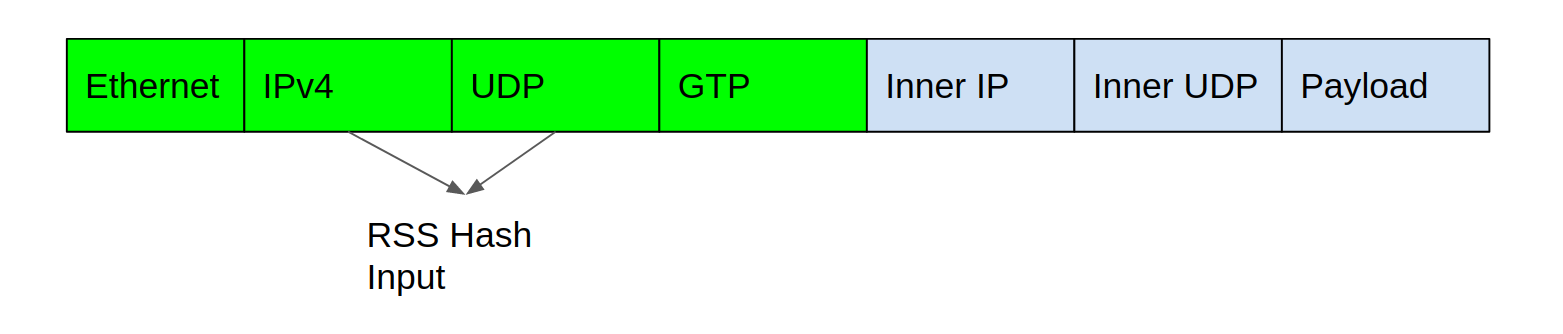
\includegraphics[width=0.7\textwidth, keepaspectratio]{./fig/Ch3DDP/noDDPpacketHashFields.png}
    \caption{Standard RSS input Fields}
    \label{figStandardRSSfields}
\end{figure}

\begin{itemize}
\item \textbf{Outer Source IP} is the RAN IP - same for all the uplink packets.
\item \textbf{Outer Source Port} In the earlier setup, this port was randomized to  get unique hash key for RSS computation. This is not a good idea as source ports are not in the control of the UPF. 
\item \textbf{Outer Destination IP} IP of the UPF - same for all the uplink packets.
\item \textbf{Outer Destination Port} is 2152 - same for all the uplink packets.
\end{itemize}
So the RSS hash key computation based on these headers will not work in our context.

\section{Alternatives \label{sectionAlternativesDDP}}
The following alternatives were explored:
\begin{itemize}
\item \textbf{Flow Director}
The 40Gbps Intel X710 NIC provides an option of inserting flow rules in the hardware itself (see \cite{flowReport}). These flow rules can be used to match different fields (including the inner payload) of the packet to make forwarding decisions. It is a better alternative than processing headers in software. However, there are two major limitations found with this approach.
\begin{itemize}
\item \textbf{Limited number of entries} Only 8k entries can be made in the flow table. The 5G use case requires us to handle UE sessions which are much larger in number. The experiments are performed for a maximum of 65536 live UE sessions. 
\item \textbf{No wildcards} Wildcard matching is not supported by the NIC. The number of flow rules could have been reduced drastically with mapping a range of UEs to a fixed core.
\end{itemize}
Due to the above limitations, the idea of using flow director was dropped. The 40Gbps NICs may support these features in future.
\item \textbf{Dynamic Device Personalization for RSS} This feature provides  the capability to parse fields of inner packet in a GTP-U packet for hash computation. This feature was exploited to get hardware based redirection and is explained in further sections.
\end{itemize}

\section{Dynamic Device Personalization \label{sectionDDP}}
Intel 40 Gbps NIC (XL710) provides the capablility to customize RSS hash key input fields \cite{ddpGuide}. RSS hash is still computed in hardware. However the fields parsed for RSS hash computation includes 
\begin{figure}[htbp]
    \centering
    \includegraphics[width=0.7\textwidth, keepaspectratio]{./fig/Ch3DDP/DDPpacketHashFields.png}
    \caption{DDP RSS input Fields}
    \label{figDDPRSSfields}
\end{figure}


\begin{itemize} 
\item \textbf{Inner Packet IP fields} Every UE has different source IP. It may not be unique for multiple sessions by the same UE. Still it has good randomness.
\item \textbf{Tunnel ID in GTP header} This field is unique for every session. 
\end{itemize}
So a combination of the above two tuples generates enough randomness for redirection of packets on different cores. 
As the name suggests, this feature/profile can be dynamically loaded and removed from the NIC during the execution of the program. There are no permanent changes made to the NIC configuration.
Note that this feature can also be used with Flow Director (discussed in section \ref{sectionAlternativesDDP}) which was not used because of the reasons mentioned.

\section{Limitations of Dynamic Device Personalization \label{sectionlimitationsDDP}}
This feature requires exact matching of all the headers for hash computation. If a field does not follow the protocol format, the packets are directed to the first queue configured on the NIC.

\begin{figure}[htbp]
    \centering
    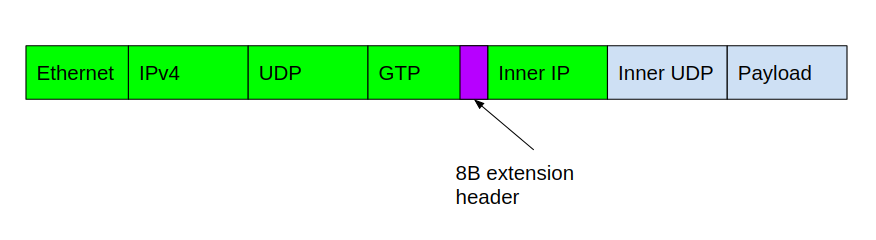
\includegraphics[width=0.7\textwidth, keepaspectratio]{./fig/Ch3DDP/ExtensionHeaders.png}
    \caption{Extension Header Limitation}
    \label{figextensionheaderLimitation}
\end{figure}

The extension header is used in our case for  providing QoS aggregate maximum bit rate (AMBR) that is allowed per session. The parsing of the GTP packet fails due to the presence of the extension header and all packets are directed to the first queue.
This is the limitation of the hardware and may be addressed in future by programmable switches or customized DDP feature prvided by hardware vendor (Intel in this case).
The experiments performed during this project are not providing different AMBRs for different sessions. AMBR is set above the incoming rate. As a workaround, no extension header is used and AMBR is implicitly assumed. The pipeline model does not have this limitation and the extension headers are used.













%    \centering
%    \includegraphics[width=0.7\textwidth, keepaspectratio]{./fig/c3f1.png}
%    \caption{DPDK: Packet movement}
%    \label{fig1c3}
%    \end{figure}
%\section{Introduction} 
%Poll Mode Drivers (PMD) are the user space network drivers. The device drivers are a piece of software which knows how to 
%interact with an external device like hard disk, CD-ROM, and NIC among others. The network drivers are the device drivers which interact with network devices like NICs. DPDK has drivers compatible with 1 Gigabit, 10 Gigabit and 40 Gigabit Intel NICS. DPDK also has drivers compatible with \emph{virtio} - a virtual device used for interacting with virtual machines.
%
%
%\section{Background: Interaction between a Driver and a Device \label{backdriver3}}
%The device and the driver store data and control information like statistics, debugging or error status at two places-
%\begin{itemize}
%    \item Base Address Registers (BARs) on the device (NICs in our case). These are primarily used to store control information.
%    \item Main Memory Locations. The data (packets) are primarily stored here. 
%    \end{itemize}
%The data is transferred with the help of
%\begin{itemize}
%        \item \textbf{Memory-Mapped IO (MMIO)} The BARs or RAM location used for data transfer are placed in the shared address space. The user process or driver can communicate with BARs or shared memory by reading or writing on these addresses. Similarly the device (NICs) can write (read) data packets to (from) these shared memory regions using DMA transfer. 
%        \item  \textbf{x86 IO ports} Data can also be transferred by writing to registers using \emph{x86 in and out instructions}. This technique is not used with modern NICs. However it is used along with MMIO in virtio implementation by writing memory addresses in IO registers in igb\_uio drivers (section \ref{uio3}).
%    \end{itemize}
%    \subsection{Transfer of Packets}
%    \subsubsection{Hardware NICs \label{nic3}}
%NICs have multiple receive and transmit queues. Incoming traffic is distributed among different receive queues by using hashing technique. Multiple transmit queues generally combine into one queue per interface before transmitting packets.
%A simple model of one receive queue and one transmit queue is assumed in the following description.   
%\begin{figure}[htbp]
%    \centering
%    \includegraphics[width=0.7\textwidth, keepaspectratio]{./fig/c3f2.png}
%    \caption{DMA descriptors \cite{ixydpdk}}
%    \label{fig2c3}
%    \end{figure}
%The driver allocates space for a circular array for holding pointers to the physical address of the data packets. These pointers are called \emph{DMA} descriptors (see Figure \ref{fig2c3}). Packets are moved by passing these descriptors between NIC and driver with the help of a head (owned by NIC) and a tail (owned by driver) pointer. 
%A buffer table (Figure \ref{fig3c3}) which maps physical addresses to virtual addresses is also maintained. This mapping is required on packet reception as the user process uses virtual addresses. The packets are processed in batches.
%\begin{figure}[htbp]
%    \centering
%    \includegraphics[width=0.7\textwidth, keepaspectratio]{./fig/c3f3.png}
%    \caption{Layout of a receive queue \cite{ixydpdk}}
%    \label{fig3c3} 
%    \end{figure}
%
%
%Transmit side is similar except for the asynchronous transfer of packets on to the links. The process returns after filling the packets on the ring. When the packets are transmitted later, the driver is notified by the movement of pointers on the circular buffer. The sent packets are subsequently freed or erased and returned back to memory pools (\ref{mempool4}). 
%\subsubsection{\emph{virtio} queues}
%\emph{virtio} queues are used to transmit data packets between host machine and virtual machines.  Packets are received/transmitted by storing them in DMA buffers (section \ref{nic3}). However virtio queues (that store DMA descriptors) consists of two rings- \emph{available} and \emph{used} (see Figure \ref{fig4c3}).
%% On the transmit side, the packets' descriptors are inserted in the 
%The \textbf{available} ring is used for receipt/transfer of packets. Once the packets are processed, the descriptors are kept in the  \textbf{used} ring . The network driver then clears the descriptors and which can then be reused.
%The \textbf{available} queue indices are written in device registers using \emph{IN/OUT} x86 instructions. 
%\begin{figure}[htbp]
%    \centering
%    \includegraphics[width=0.7\textwidth, keepaspectratio]{./fig/c3f4.png}
%    \caption{Virtio Queues \cite{ixydpdk}}
%    \label{fig4c3} 
%    \end{figure}
%The virtio queues are not exclusively used for packet transfers. For example, virtio queues are also used for reading files from disk. The transmit function prepends a header to the network data. This header helps the driver in differentiating network packets from other devices' data.     
%
%\section{Design of important PMDs}
%\subsection{igb\_uio \label{uio3}}
%DPDK uses \emph{uio} kernel subsystem to build \emph{igb\_uio}\cite{memblogdpdk2} driver. This driver is used for both virtio and hardware NICs \cite{ixydpdk}. \emph{uio} provides full access to the shared registers and shared memory by memory mapping these regions into files. These files are located in \emph{sysfs} virtual-filesystem (VFS). \emph{sysfs} treats an external device as a file.
%\subsection{vfio-pci-driver}
%DPDK uses \emph{vfio} kernel subsystem to build \emph{vfio-pci} driver. vfio provides IOMMU support for virtualized environments. IOMMU is a memory translation unit present on NICs  which directly maps guest virtual addresses to host physical addresses. This enables NICs to perform DMA directly and guest VMs can interact with devices using guest virtual addresses. 
%\subsection{Software PMDs \label{softpmd3}} 
%DPDK also has PMDs which do not require kernel subsystems like uio or vfio. These PMDs are built over packet capture libraries
%like \emph{libpcap} and \emph{AF\_PACKET} \cite{afpacket} sockets. The packet capture framework allows DPDK to work with any hardware by providing raw packets to the driver. 
%
%
%
%
%
%\section{Configuration and Device Statistics}
%DPDK PMDs provide APIs for configuring and collecting device statistics from NICs (Figure \ref{fig5c3}).
%\begin{figure}[htbp]
%    \centering
%    \includegraphics[width=0.7\textwidth, keepaspectratio]{./fig/c3f5.png}
%    \caption{Control APIs}
%    \label{fig5c3} 
%    \end{figure}
%\subsection{Configuration \label{config3}}
%Depending on the capability of hardware NICs, the NICs can be configured for
%\begin{itemize}
%    \item \textbf{Offloading Calculations} - Checksums, CRC checks, VLAN tag processing among others.
%    \item \textbf{Directing Traffic} - Destination lookup and making forwarding decisions like dropping packets, diverting it to a specific queue,  packet encapsulations for tunnel offloads (IPv6 packet inside a IPv4 packet for transmitting on an IPv4 compatible link) and so on.
%\end{itemize}
%This is performed with the help of APIs which are present in Flow Library\cite{progguide}. 
%
%\subsection{Device Statistics}
%PMDs provide APIs for collecting statistics on the network traffic. The statistics include but are not limited to number of incoming packets, number of transmitted packets, packet drop rate etc. The extended statistics API is used for getting statistics which are unique to a device.
%
%It is the responsibility of application developer to use these statistics or configure the hardware if required. The PMDs act as the translators between application and the hardware.
%


